\documentclass[letterpaper,twocolumn,10pt]{article}
\usepackage[margin=0.75in]{geometry}

\usepackage{graphicx}
\newcommand{\vB}{\mbox{$\bf v$}}
\newcommand{\xB}{\mbox{$\bf x$}}
\newcommand{\yB}{\mbox{$\bf y$}}
\newcommand{\JB}{\mbox{$\bf J$}}
\newcommand{\RB}{\mbox{$\bf R$}}
\newcommand{\WB}{\mbox{$\bf W$}}
\newcommand{\PB}{\mbox{$\bf P$}}
\newcommand{\MB}{\mbox{$\bf M$}}
\newcommand{\IB}{\mbox{$\bf I$}}
\newcommand{\SG}{\mbox{$\bf \Sigma$}}
\newcommand{\sG}{\mbox{$\bf \sigma$}}
\newcommand{\etal}{{\em et al}}
\begin{document}

\title{\bf 
Simple FEMs aren't as good as we thought: \\
  experiences developing EIDORS v3.3%
}

\author{Andy Adler$^{1}$,
        Andrea Borsic$^{2}$,
        Nick Polydorides$^{3}$,
        William R B Lionheart$^{4}$}
\date{}
\maketitle

\begin{abstract}
This paper covers two topics. First, we announce
EIDORS version 3.3, and clarify the new features and
changes to the software.
Next,
we discuss accuracy limitations to the single-order
tetrahedral finite element models that are used
in much EIT research. Specifically, the accuracy
of simulated voltages is expored as a function
of mesh density and electrode refinement.
A conductive object was simulated moving in a 
circular tank, using adaptive mesh refinement
around the object. Images were reconstructed
using difference EIT and compared to those from
a saline tank phantom.
FEM accuracy may be partially addressed using
dual model solvers, for which EIDORS v3,3
provides support.
Briefly, the new version also includes:
1) interfaces to FEM generation (distmesh, netgen) and 
  dual model solvers
2) new algorithms (total variation, electrode movement solver,
  temporal solvers) 
3) a data repository with several contributed models, clinical
   and experimental data sets
4) faster algorithms with better caching, and
5) improved graphics and extensive tutorials
\end{abstract}

\section{Introduction}

\section{EIDORS version 3.3}

EIDORS (Electrical Impedance Tomography and Diffuse Optical
 Tomography Reconstruction Software) is an open source
suite of software for reconstruction of images in soft 
field tomography modalities. The earlist version was made
available in 1999 and provided support for 2D EIT (Vauhkonen).
Subsequently, support for 3D EIT was provided (Polydorides) in 
2000. In 2005, EIDORS was refactored to allow ``pluggability''
-- easy incorporation of contirubted algorithms and 
functionality -- as part of EIDORS version $3$ (while the
previous releases were renamed $v1$ and $v2$, respectively). 
Version $3.0$ was released in 2005, $v3.1$ in 2006 (and described
in Adler and Lionheart, 2006), $v3.2$ in 2007, and $v3.3$
(described in this paper). Many new features have been added;
in terms of lines of code, $v2.0$ has 3715, $v3.0$ has 10685
and $v3.3$ has 27774 (with another 5940 in tutorials).

The following high-level new features are part of EIDORS v3.3:

\newcounter{Ictr}
\begin{list}{\bf \arabic{section}.\arabic{Ictr}}
  {\leftmargin=0.0em \itemindent=2.0em
%   \topsep= 0.0\baselineskip
%   \itemsep=-0.0em
    \listparindent=1.0em \parsep=-0.0em
    \usecounter{Ictr}}
\item {\bf interfaces to FEM generation}

Interfaces to Netgen, Distmesh

\item {\bf support for dual model solvers}

\item {\bf new algorithms}
 (total variation, electrode movement solver,
  temporal solvers)

\item {\bf data repository}
 with several contributed models, clinical
   and experimental data sets

\item {\bf faster algorithms}
   PDIPM, Jacobian, with better caching

\item {\bf improved graphics and extensive tutorials}

\end{list}

\section{Dual Model solvers}

\begin{figure}[tbh]
\begin{center}
 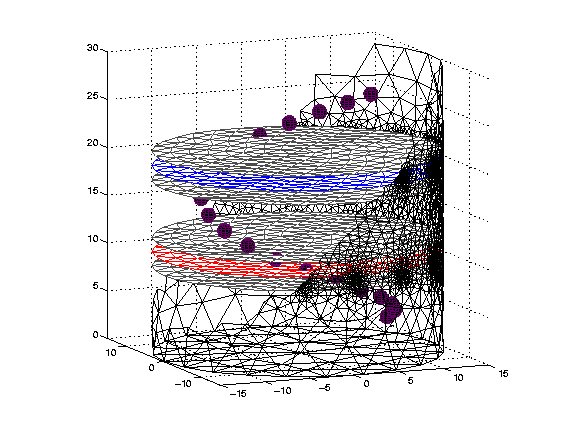
\includegraphics[width= 0.45\textwidth]{../../tutorial/dual_model/centre_slice02a.png}
\caption{ \label{fig:dual_model}
\small
Netgen model of a 2�16 electrode tank. The positions of the simulated
conductive target moving in a helical path are shown in purple. The
3D fine model is shown (cropped). The upper (blue) and lower (red)
layers corresponding to the geometry of the coarse model are shown. The
z direction limits of the coarse model are shown in grey.
}
\end{center}
\end{figure}

\begin{figure}[tbh]
\begin{center}
 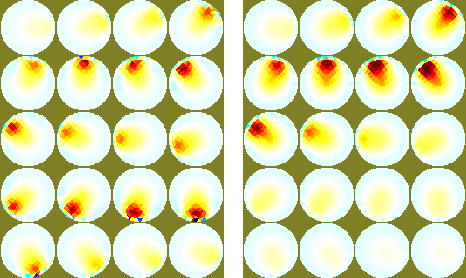
\includegraphics[width= 0.45\textwidth]{figs/centre_slice04a_crop.png}
\caption{ \label{fig:dual_model_reconst}
\small
Reconstructed images of a target moving in a helical pattern using
difference reconstruction models.
{\em Left} reconstruction model with  $z_{depth}=\infty$
{\em Right} reconstruction model with $z_{depth}= 0.1\times \mbox{scale}$
at lower position in Fig. \ref{fig:dual_model}
}
\end{center}
\end{figure}

A dual reconstruction model uses a fine finite element
model (FEM) to implement the forward solution (voltages
at electrodes), and a coarse mesh for the inverse
solution. For example, a dual model may be used to 
represent the conductivity change in a layer
of a 3D plane (ie. Fig. \ref{fig:dual_model}).
Given a forward model, $F$,
which calculates a voltage measurement vector, $\vB$, from
a forward (fine) model conductivity element vector, $\sG_f$, we
have $\vB = F( \sG_f )$. The reconstruction (coarse)
model is defined on square elements $\sG_r$ related by
a coarse to fine projection matrix $\PB$, where $\sG_f = \PB \sG_r$.

Dual meshes may be used in several applications:
\begin{list}{$\circ$} %{\textbullet}
  {\leftmargin=1.0em \itemindent=-0.0em
    \topsep=0.0\baselineskip
    \itemsep=-0.4\baselineskip}
\item
   corresponding meshes
\item
   elem to node (nodal solvers)
\item
   $2\frac{1}{2}$ solvers
\item
   constraining parameter choices (ie having one parameter
      for out of plane conductivity to prevent the system from
      "pushing" artefacts there.
\item
   solving to a rasterized mesh as in GREIT
\end{list}


Dual meshes have been used by many EIT groups (FIX THIS STUFF)
\\
- We used an interpolation method on two meshes since the early code in the Fortran code Recon started by me and contiued by Kevin Paulson at Brookes. It seemed to trivial to make a big deal our of it. The way we did it used a mesh correspondence array. 
\\
- Later on the Dartmouth group also stumbled on the idea and there was a paper by the similarly named Keith Paulsen. Although I thought there was nothing very remarkable there.
\\
- As I remember Marko used two meshes in his code that was the original 2D Eidors. Is that in his thesis?
\\
- I am pretty sure that the UCL optimal tomography people also do it in TOAST, and so now doubt Hamid uses it in EIT too.

\section{FEM accuracy}

Finite Element Model (FEM) accuracy is normally considered
from the point of view of voltage errors between FEM and
physical phantom. While this is correct, any errors may be explained
by small details in the phantom which are not considered
in the model. Here we consider FEM accuracy from the
approach of looking at small changes in the model and their
consequences on time difference EIT images.

The easiest (and most common) way to simulate a moving target
in a medium is to use a single FEM to select and then interpolate
which elements are part of that target. Fig. \ref{fig:fem1}
shows a 2062 element FEM created by distmesh, with mesh
refinement near the electrodes. Sixteen electrodes are
simulated using a Sheffield-type adjacent stimulation and
measurement. For each simulated target position (blue), the
fraction of each element filled by the target is calculated
and the conductivity change is scaled by this fraction.

\begin{figure}[tbh]
\begin{center}
 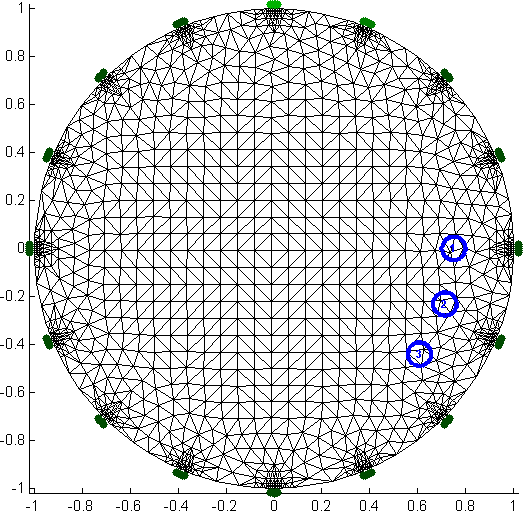
\includegraphics[width= 0.24\textwidth]{figs/fig1a.png}
 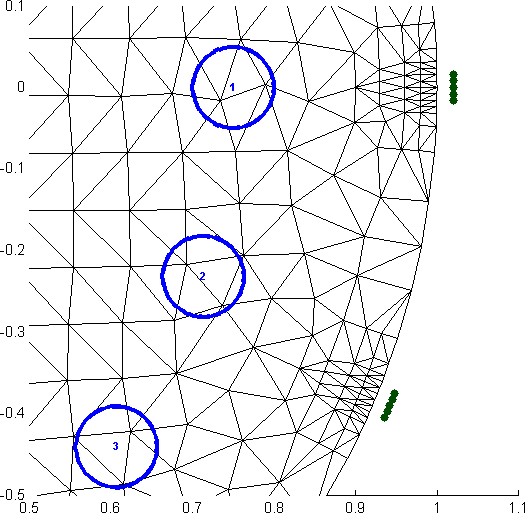
\includegraphics[width= 0.24\textwidth]{figs/fig1b.png}
\caption{ \label{fig:fem1}
\small
Simulation FEM and simulated target positions in blue
{\em Left} full scale mesh.
{\em Right} mesh magnified near target positions 
}
\end{center}
\end{figure}

Images are reconstructed of the three target positions
in Fig. \ref{fig:fem1_images} using a one-step regularized
GN image reconstruction. There is no change to
the underlying FEM, and thus no noise in the images.

\begin{figure}[tbh]
\begin{center}
 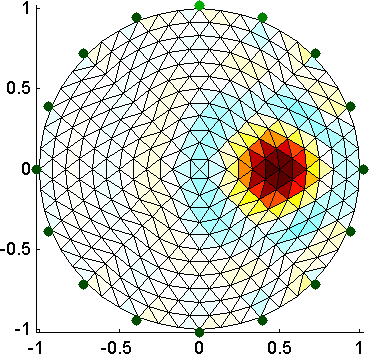
\includegraphics[width= 0.15\textwidth]{figs/fig2a.png}
 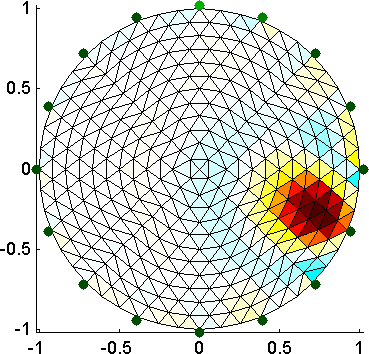
\includegraphics[width= 0.15\textwidth]{figs/fig2b.png}
 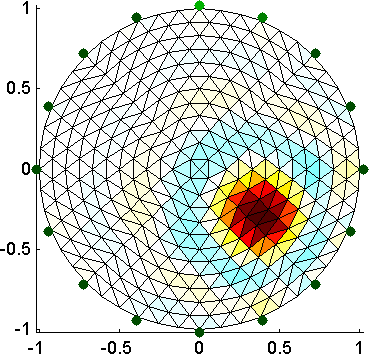
\includegraphics[width= 0.15\textwidth]{figs/fig2c.png}
\caption{ \label{fig:fem1_images}
\small
Images reconstructed of targets simulated from
interpolated shapes in Fig. \ref{fig:fem1}, from
left to right, targets 1 to 3.
}
\end{center}
\end{figure}

However, the best way to simulate a moving target is
create a target region within the FEM and to remesh around
it. This means that the mesh changes between each
target position, not only near the target, but throughout
the FEM due to the propagation of changes in triangularization.

\begin{figure}[tbh]
\begin{center}
 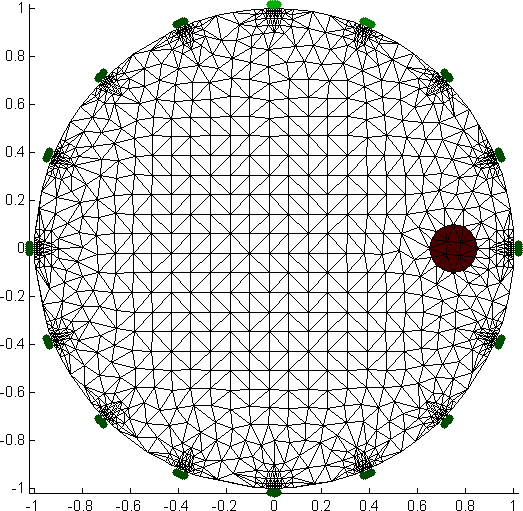
\includegraphics[width= 0.20\textwidth]{figs/fig3a-2062e.png}
 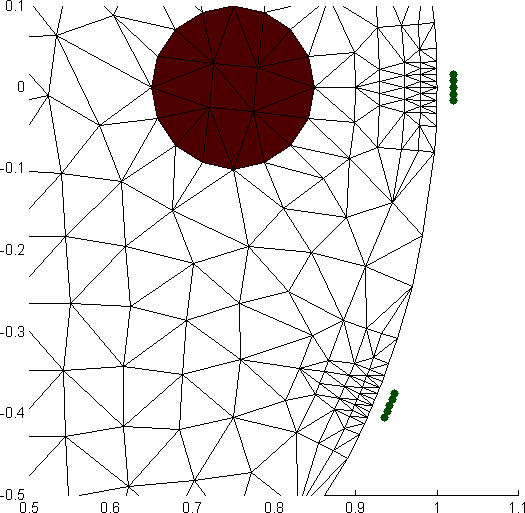
\includegraphics[width= 0.20\textwidth]{figs/fig3b-2062e.png}
 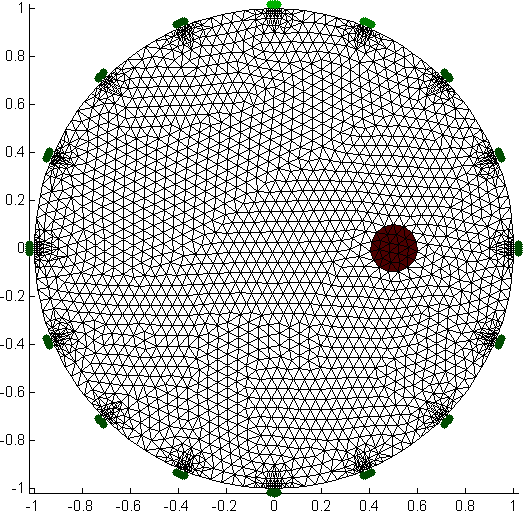
\includegraphics[width= 0.20\textwidth]{figs/fig3a-4226e.png}
 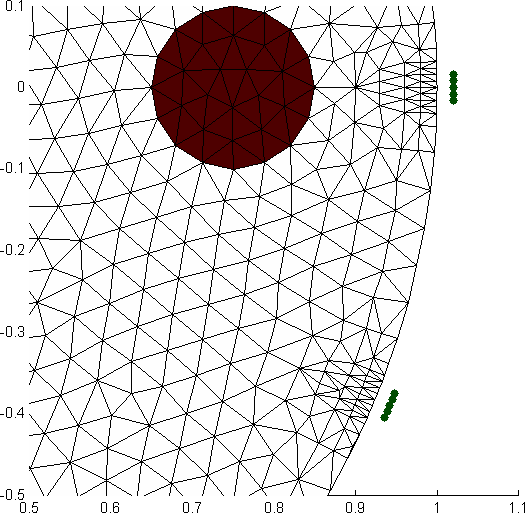
\includegraphics[width= 0.20\textwidth]{figs/fig3b-4226e.png}
 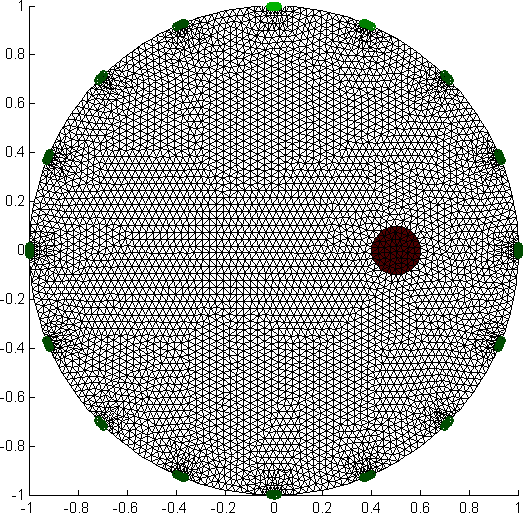
\includegraphics[width= 0.20\textwidth]{figs/fig3a-8909e.png}
 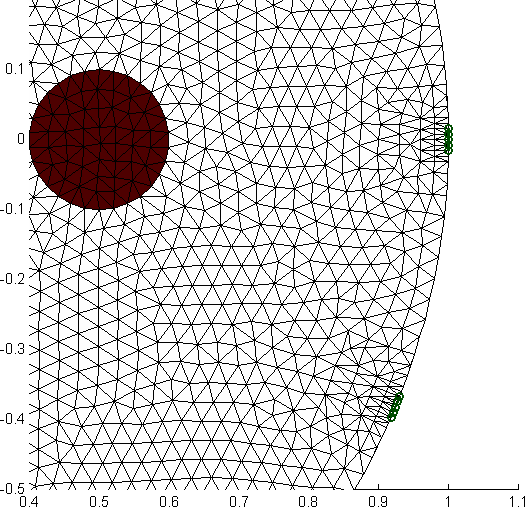
\includegraphics[width= 0.20\textwidth]{figs/fig3b-8909e.png}
\caption{ \label{fig:fem2}
\small
Simulation FEM and simulated target positions in blue
{\em Left} full scale mesh.
{\em Right} mesh magnified near target positions 
{\em Top} FEM with 2062 elements,
{\em Middle} FEM with 4226 elements,
{\em Bottom} FEM with 8909 elements,
}
\end{center}
\end{figure}

Using distmesh, FEMs were created of a homogeneous phantom
(like that of Fig. \ref{fig:fem1}), and of three phantoms
with inset targets at corresponding to the positions in
that figure.  Fig. \ref{fig:fem2} shows the mesh at the
first target position. Three different levels of mesh
refinement are shown.

Based on these simulations, we reconstruct images
using a simple 576 element mesh with point electrodes
(Fig. \ref{fig:fem2_images}. In the coarse (2062 element)
and to some extent in the medium refinement (4226 element) 
mesh, there are large artefacts near the electrodes which
dramatically disturb the image clarity.

\begin{figure}[tbh]
\begin{center}
 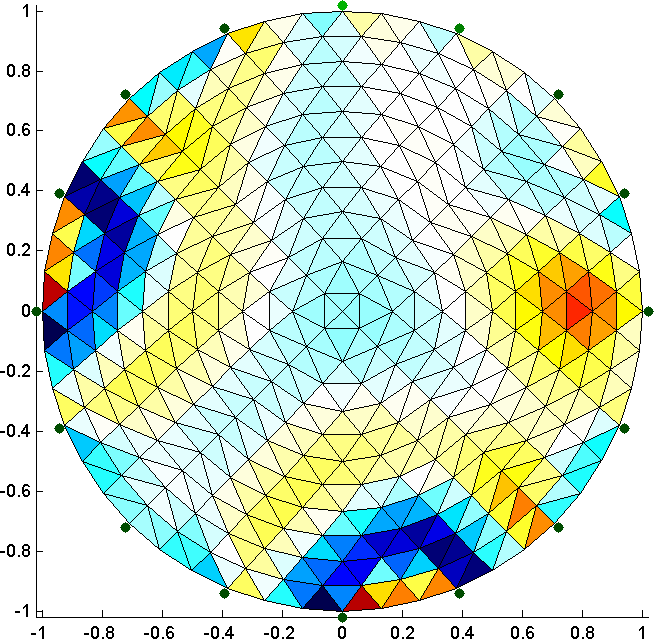
\includegraphics[width= 0.15\textwidth]{figs/fig4a-2062e.png}
 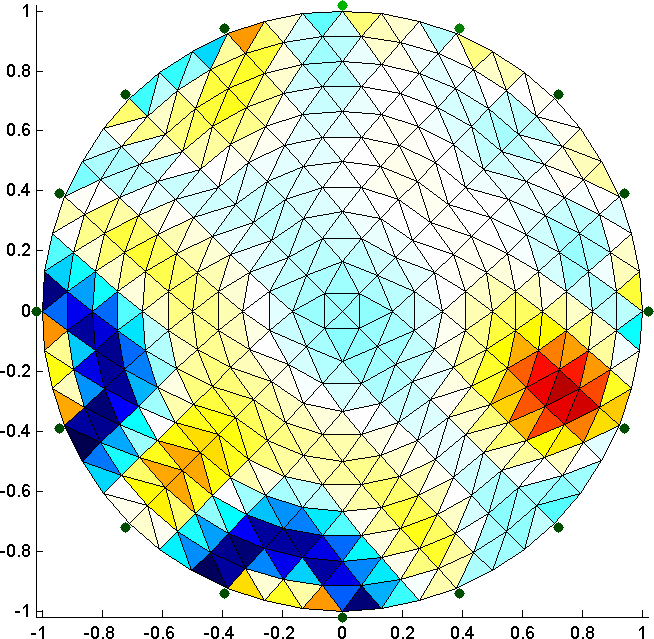
\includegraphics[width= 0.15\textwidth]{figs/fig4b-2062e.png}
 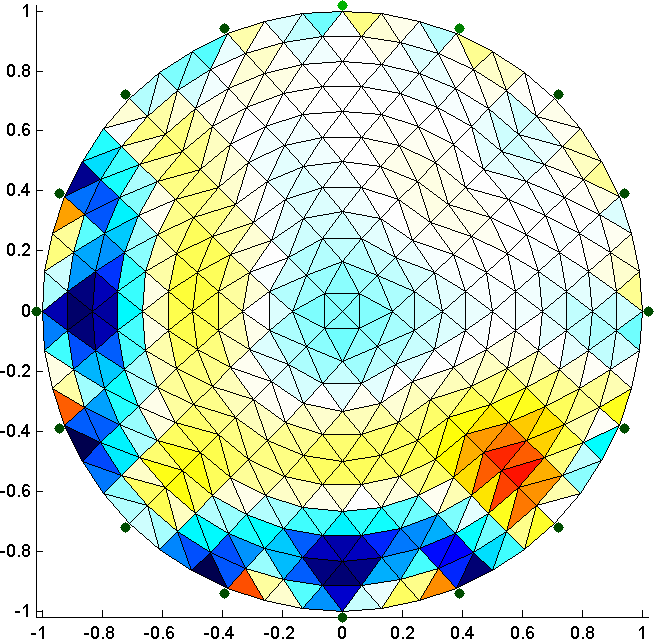
\includegraphics[width= 0.15\textwidth]{figs/fig4c-2062e.png}
 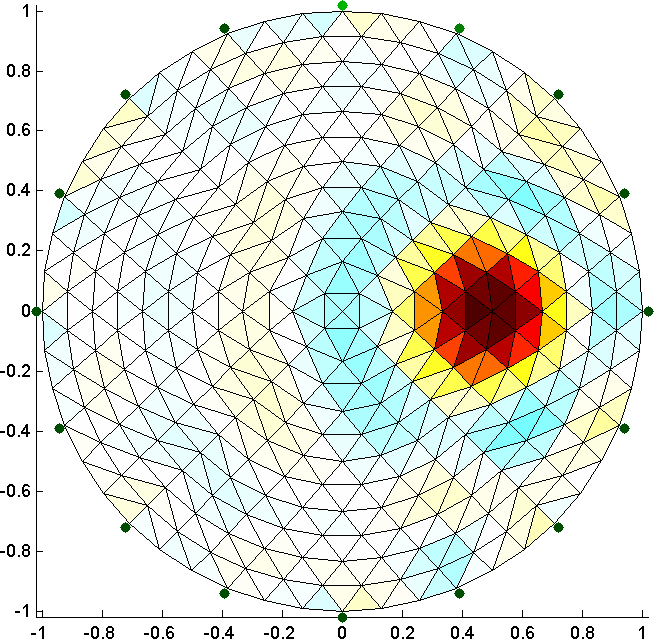
\includegraphics[width= 0.15\textwidth]{figs/fig4a-4226e.png}
 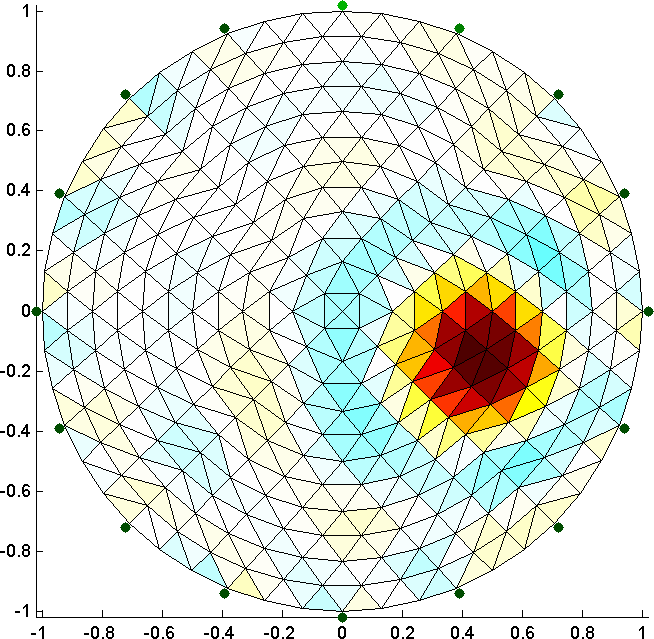
\includegraphics[width= 0.15\textwidth]{figs/fig4b-4226e.png}
 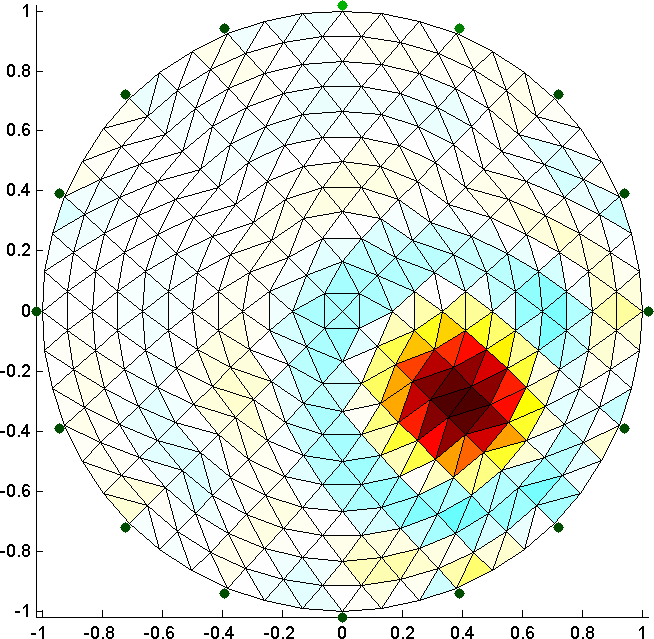
\includegraphics[width= 0.15\textwidth]{figs/fig4c-4226e.png}
 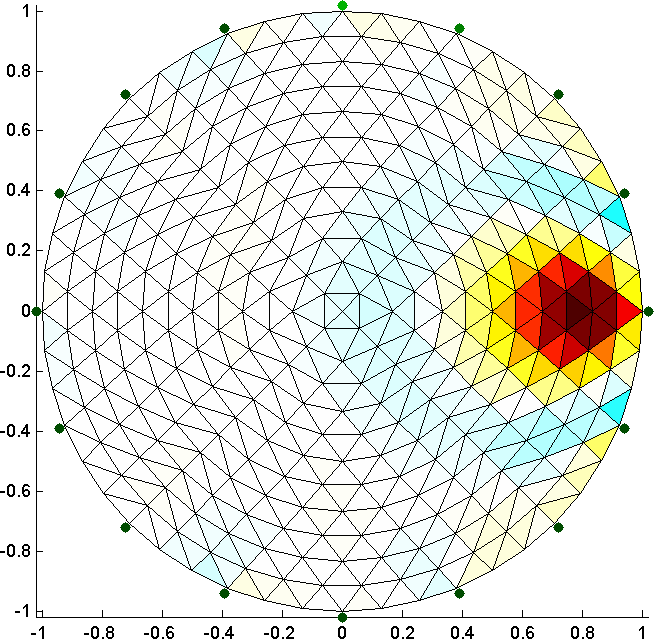
\includegraphics[width= 0.15\textwidth]{figs/fig4a-8909e.png}
 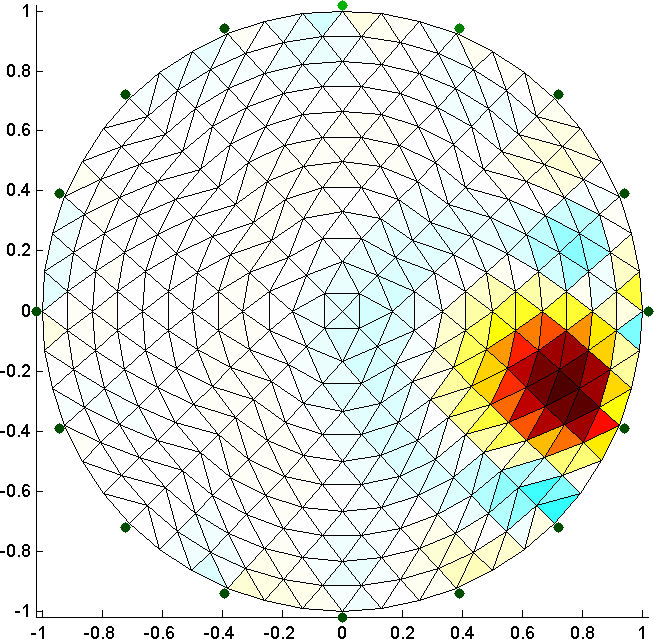
\includegraphics[width= 0.15\textwidth]{figs/fig4b-8909e.png}
 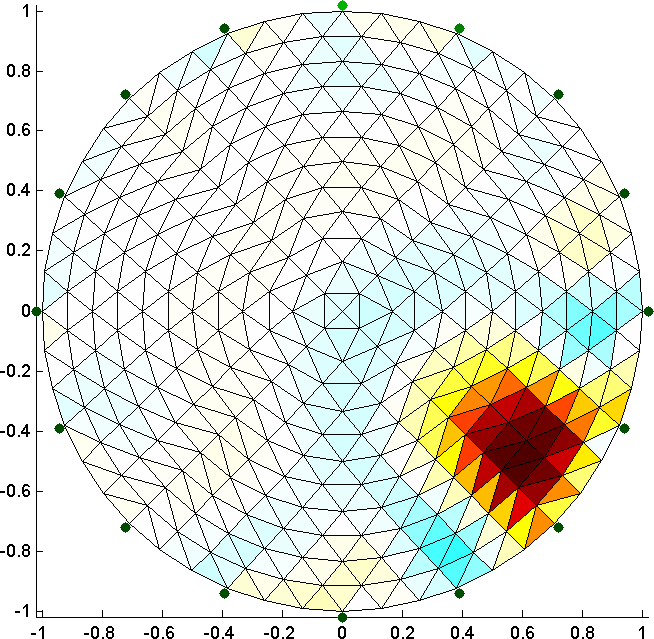
\includegraphics[width= 0.15\textwidth]{figs/fig4c-8909e.png}
\caption{ \label{fig:fem2_images}
\small
Images reconstructed of targets simulated from
interpolated shapes in Fig. \ref{fig:fem2}, from
left to right, targets 1 to 3.
{\em Top} FEM with 2062 elements,
{\em Middle} FEM with 4226 elements,
{\em Bottom} FEM with 8909 elements,
}
\end{center}
\end{figure}

TODO
\\
- compare to tank images
\\
- discuss results

\end{document}

